\documentclass{beamer}

%% Set biblatex as bibliography manager, biblatex > bibtex
\usepackage[backend=biber, style=ieee]{biblatex} % Referencias
\usepackage{graphicx} % Allows including images
\usepackage{booktabs} % Allows the use of \toprule, \midrule and \bottomrule in tables
\usepackage{siunitx}
\usepackage{lipsum}


\definecolor{colorIPN}{RGB}{108 29 69} % Pantone 222 C\\
\definecolor{colorUPIITA}{HTML}{BAB100}
\definecolor{darkGray}{RGB}{25 25 25}

\mode<presentation> {
	
	% The Beamer class comes with a number of default slide themes
	% which change the colors and layouts of slides. Below this is a list
	% of all the themes, uncomment each in turn to see what they look like.
	
	\usetheme{Madrid}
	%	Other themes are: AnnArbor, Antibes, Bergen, Berkeley, Berlin, Boadilla, CambridgeUS, Copenhagen, Darmstadt, Dresden, Frankfurt,Goettingen, Hannover, Ilmenau, JuanLesPins, Luebeck, Madrid, Malmoe, Marburg, Montpellier, PaloAlto, Pittsburgh, Rochester, Singapore, Szeged, Warsaw
	
	% As well as themes, the Beamer class has a number of color themes
	% for any slide theme. Uncomment each of these in turn to see how it
	% changes the colors of your current slide theme.
	
	\usecolortheme[named=colorIPN]{structure}
	%	Other color themes are: albatross, beaver, beetle, crane, dolphin, dove, fly, lily, orchid, rose, seagull, seahorse, whale, wolverine
	
	%	\setbeamertemplate{footline} % To remove the footer line in all slides uncomment this line
	%	\setbeamertemplate{footline}[page number] % To replace the footer line in all slides with a simple slide count uncomment this line
	
	%	\setbeamertemplate{navigation symbols}{} % To remove the navigation symbols from the bottom of all slides uncomment this line
}


\usepackage{siunitx}
\usepackage{lipsum}
\addbibresource{References.bib}

%----------------------------------------------------------------------------------------
%	PORTADA
%----------------------------------------------------------------------------------------

\title[Short title]{Full title} % The short title appears at the bottom of every slide, the full title is only on the title page
\subtitle{Subtitle}

% Primera opción
\author[name]{Full Name\\\medskip % Your name
	\texttt{politecnico-upiitense@alumno.ipn.mx}}% Your email address}

% Your institution as it will appear on the bottom of every slide, may be shorthand to save space
\institute[UPIITA-IPN]{\textit{Instituto Politécnico Nacional}\\\medskip Unidad Profesional Interdisciplinaria en Ingeniería y Tecnologías Avanzadas \\ % Your institution for the title page
}
\date{\today} % Date, can be changed to a custom date

\logo{\href{https://www.upiita.ipn.mx/}{
\includegraphics[height=10mm]{images/logo_upiita_oro}}}

%%%%%%%%%%%%%%%%%%%%%%%%%
% If you don't want the background image in the first slide put this code after the first frame.
\usepackage{background}
%\backgroundsetup{
%	placement=center,
%	scale=4,
%	contents={DRAFT},
%	opacity=1
%}
%\setbeamertemplate{background}{\BgMaterial}
\setbeamertemplate{background}{
	\tikz[overlay,remember picture]
	\node[opacity=0.25]at (current page.center)
	{
\includegraphics[width=5cm]{images/LOGO POLI PANTONE 222 C}};
}
%%%%%%%%%%%%%%%%%%%%%%%%%

\begin{document}
	
	% Change background color to all subsequent frames
%	\setbeamercolor{background canvas}{bg=black!90}

	\begin{frame}
		\thispagestyle{empty} % Hide headers and footers
		\titlepage % Print the title page as the first slide
	\end{frame}
	%------------------------------------------------
	%	CONTENIDO
	%------------------------------------------------
	\begin{frame}
		\frametitle{Contenido} % Table of contents slide, comment this block out to remove it
		\tableofcontents 
	\end{frame}
	%------------------------------------------------
	%------------------------------------------------
	\begin{frame}
		\section{Resumen}
		\frametitle{Resumen} 
		\framesubtitle{Palabras clave}
		\label{Resumen}
		
		En este archivo se muestran algunos formatos de láminas que pudieran ser de utilidad o servir de referencia.
		
		\vspace{5mm}
		
		%\Palabras clave
		\label{Keywords}
		\textbf{{\large Palabras clave:}} beamer, presentación
	\end{frame}
	%------------------------------------------------
	\begin{frame}
		\section{Mucho texto}
		\frametitle{Mucho texto}
		\framesubtitle{Ejemplicación de una lámina con mucho texto}
		\lipsum[1]
	\end{frame}
	%------------------------------------------------
	\begin{frame}
		\section{Poco texto + imagen}
		\frametitle{Párrafo pequeño más una imagen}
		\lipsum[2][1-5]
		
		\begin{center}
			
\includegraphics[height=50mm]{images/logo_upiita_oro}
		\end{center}
	\end{frame}
	%------------------------------------------------
	\begin{frame}
		%\section{Poco texto + imagen}
		\frametitle{Párrafo pequeño más una imagen lado a lado}
		
		\begin{minipage}{\textwidth}
			\begin{minipage}{0.60\textwidth}
				\lipsum[5][1-8]
			\end{minipage}
			\hfill
			\begin{minipage}{0.35\textwidth}
				
\includegraphics[height=40mm]{images/logo_upiita_oro}
			\end{minipage}
		\end{minipage}
	\end{frame}
	%------------------------------------------------
	\begin{frame}
		\section{Lista}
		\frametitle{Lista}
		\frametitle{Párrafo pequeño más una lista}
		\lipsum[3][1-5]
		
		\SetLipsumSentenceListSurrounders{\begin{itemize}}{\end{itemize}}
		\SetLipsumSentenceListItemStart{\item}
		\lipsum[3][6-9]
%		\begin{itemize}
%			\item xzczc
%			\item hk
%			\item sadasd
%		\end{itemize}
	\end{frame}
	%------------------------------------------------
	\begin{frame}
		\section{Imagen y una tabla}
		\frametitle{Imagen y una tabla}
		\framesubtitle{Imagen al lado de una tabla}
		
		% Jugar con los valores de los 2 minipage, el tamaño de la imagen, el espacio horizontal entre los minipage y ancho de las columnas.
		\begin{minipage}{\textwidth}
			\begin{minipage}{0.39\textwidth}
				\centering
				
\includegraphics[height=60mm]{images/logo_upiita_oro}
%				\caption{Algo acerca de la imagen}
			\end{minipage}
			\hspace{15mm}%\quad%\qquad%\hfill
			\begin{minipage}{0.45\textwidth}
				{\tiny \begin{tabular}{c p{40mm}}
						S\textsubscript{ex} & \lipsum[4][1-5]\\
						M\textsubscript{1} & \lipsum[4][6-10] \\
						M\textsubscript{2} & \lipsum[4][11-15] \\
				\end{tabular}}
			\end{minipage}
		\end{minipage}
	\end{frame}
	%------------------------------------------------
	\begin{frame}
		\section{Tabla grande}
		\frametitle{Tabla grande}
		\framesubtitle{Proceso Analítico Jerárquico}
		
		\begin{table}[!ht]
			\caption{Matriz de criterios normalizada}
			\resizebox{\textwidth}{!}{%
				\begin{tabular}{cccccccccc}
					\toprule
					Criterios &  Cr1   &  Cr2   &  Cr3   &  Cr4   &  Cr5   & Cr6  &  Cr7   &   TF   &      VP      \\ \midrule
					Cr1    & 0.1053 & 0.1875 & 0.1875 & 0.1429 & 0.1667 & 0.04 & 0.0588 & 0.8887 & {[}0.127{]}  \\ %
					Cr2    & 0.1053 & 0.1875 & 0.1875 & 0.1429 &  0.25  & 0.24 & 0.2353 & 1.3485 & {[}0.1926{]} \\ %
					Cr3    & 0.1053 & 0.1875 & 0.1875 & 0.1429 &  0.25  & 0.24 & 0.2353 & 1.3485 & {[}0.1926{]} \\ %
					Cr4    & 0.1053 & 0.1875 & 0.1875 & 0.1429 & 0.0833 & 0.12 & 0.1176 & 0.9441 & {[}0.1349{]} \\ %
					Cr5    & 0.0526 & 0.0625 & 0.0625 & 0.1429 & 0.0833 & 0.12 & 0.1176 & 0.6414 & {[}0.0916{]} \\ %
					Cr6    & 0.3158 & 0.0938 & 0.0938 & 0.1429 & 0.0833 & 0.12 & 0.1176 & 0.9672 & {[}0.1382{]} \\ %
					Cr7    & 0.2105 & 0.0938 & 0.0938 & 0.1429 & 0.0833 & 0.12 & 0.1176 & 0.8619 & {[}0.1231{]} \\ \midrule
					Suma    & 1.0001 & 1.0001 & 1.0001 & 1.0003 & 0.9999 & 1.0  & 0.9998 & 7.0003 &   {[}1.{]}   \\ \bottomrule
				\end{tabular}
			}
		\end{table}	
	\end{frame}

	% ¿Como crear esta tabla de forma automática?
	% https://github.com/hasecilu/AHPtableGenerator

	%------------------------------------------------
	\begin{frame}
		\section{Hipervínculos}
		\frametitle{Hipervínculos}
		\framesubtitle{De forma escondida en texto y mostrando la url}
		
		Puedes dar clic en el \href{https://bit.ly/3mhwQhI}{``clickbait''}.
		\vspace{25mm}
		
		O puedes mostrar la url: \url{https://bit.ly/3mhwQhI}
		
	\end{frame}
	%------------------------------------------------
	\begin{frame}
		\section{Robot antropomórfico}
		\frametitle{Robot antropomórfico}
		\begin{minipage}{\textwidth}
			\begin{minipage}{0.5\textwidth}
				%				\centering
				\begin{figure}[!ht]
					\centering
					%					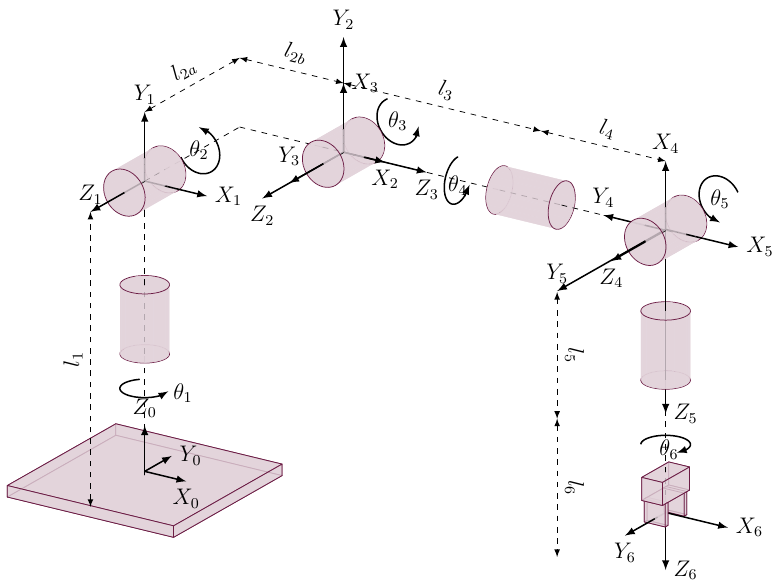
\includegraphics[height=65mm]{images/antro2}
					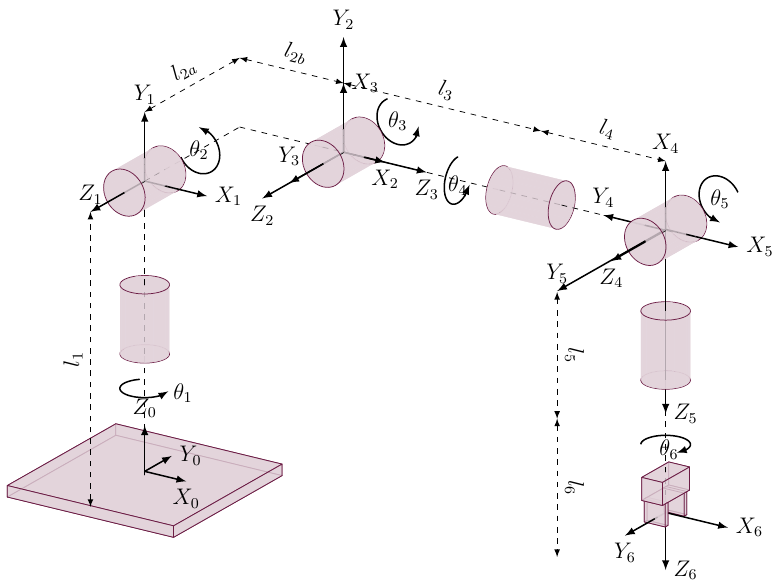
\includegraphics[width=55mm]{images/antro2}
					\caption{Diagrama cinemático del robot antropomórfico}
				\end{figure}
			\end{minipage}
			%\hspace{15mm}%\quad%\qquad%\hfill
			\quad
			\begin{minipage}{0.45\textwidth}
				Esta imagen se creó usando el el paquete sketch-lib de Alex Dumitrache (\url{https://alexdu.github.io/sketch-lib/}), este programa se usa en consola compilando un archivo .sk y genera un código de \LaTeX usando Tikz que al compilarse se genera el robot, se puede cambiar el color en el archivo .tex generado. Se puede insertar el pdf generado o convetir a imagen para quitar el fondo blanco.
			\end{minipage}
		\end{minipage}
	\end{frame}
	%------------------------------------------------
	\begin{frame}   
		\section{Ecuación grande}
		\frametitle{Ecuación grande}
		\framesubtitle{Sin cambiar el tamaño y cambiándolo (comparación)}
		
		\begin{equation} 
			R_6^3 =
			\begin{vmatrix}
				C(q_4)C(q_6)C(q_5)-C(q_4)C(q_6) & -C(q_4)S(q_6)S(q_5)-S(q_4)C(q_6) & -C(q_4)C(q_5) \\
				S(q_4)C(q_6)S(q_5)+C(q_4)S(q_6) & -S(q_4)S(q_6)S(q_5)+C(q_4)C(q_6) & -S(q_4)C(q_5) \\
				C(q_5)C(q_6)                    & -C(q_5)S(q_6)                    & S(q_5)
			\end{vmatrix}
		\end{equation}
	
		% Usar el asterisco * (sin albur) hace que desaparezca la enumeración de la ecuación
		\begin{equation*} 
			\resizebox{\textwidth}{!}{
				$	% Habilitamos el modo matemático porque \resizebox está en modo texto
				R_6^3 =
				\begin{bmatrix}
					C(q_4)C(q_6)C(q_5)-C(q_4)C(q_6) & -C(q_4)S(q_6)S(q_5)-S(q_4)C(q_6) & -C(q_4)C(q_5) \\
					S(q_4)C(q_6)S(q_5)+C(q_4)S(q_6) & -S(q_4)S(q_6)S(q_5)+C(q_4)C(q_6) & -S(q_4)C(q_5) \\
					C(q_5)C(q_6)                    & -C(q_5)S(q_6)                    & S(q_5)
				\end{bmatrix}
			$
			}
		\end{equation*}

	\end{frame}
	%------------------------------------------------
	\begin{frame}[t,allowframebreaks]
		\section{Elementos muy grandes}
		\frametitle{Elementos muy grandes}
		\framesubtitle{Ocupan varias páginas pero no es necesario crear diferentes frames}
		% Mucho texto en láminas no está chido =(
		\lipsum[6-9]
	\end{frame}
	%------------------------------------------------
%	\begin{frame}[t,allowframebreaks]
%		\section{Referencias}
%		\frametitle{Referencias}
%		\printbibliography
%	\end{frame}

% https://www.youtube.com/watch?v=GAVXVkcpbG0

\end{document}